% Two-page project write-up. Build:  cd report/writeup && pdflatex writeup.tex  (twice)
% The numbers in \newcommand below come from results/tables/*_summary.md.
\documentclass[10pt,a4paper]{article}
\usepackage[a4paper,margin=1.55cm,top=1.3cm,bottom=1.4cm]{geometry}
\usepackage[T1]{fontenc}
\usepackage[sc]{mathpazo}
\linespread{1.02}
\renewcommand{\ttdefault}{pcr}
\usepackage{amsmath,booktabs,graphicx,tabularx,xcolor,microtype}
\usepackage[hidelinks]{hyperref}
\usepackage[font=small,labelfont=bf,skip=3pt]{caption}
\usepackage{enumitem}
\usepackage{titlesec}
\titleformat{\section}{\normalsize\bfseries\color{accent}}{\thesection.}{0.4em}{}
\titlespacing*{\section}{0pt}{5pt}{2pt}
\setlist{nosep,leftmargin=1.2em}
\setlength{\parskip}{2.5pt}
\setlength{\parindent}{0pt}
\definecolor{accent}{HTML}{184F95}
\renewcommand{\arraystretch}{1.12}

% ---- poromechanics results (results/tables/poromechanics_summary.md) ----
\newcommand{\poroPaperP}{2.1e-1}     % rel. L2 error of P, paper recipe (median)
\newcommand{\poroOursP}{2.2e-4}      % rel. L2 error of P, enriched (median)
\newcommand{\poroInvPaper}{1/5}      % inverse, paper recipe: seeds within 1%
\newcommand{\poroInvOurs}{5/5}       % inverse, enriched, clean: seeds within 1%
\newcommand{\poroInvErr}{6e-5}       % median error in c, enriched, clean

\begin{document}

\begin{center}
{\Large\bfseries Physics-Informed Neural Networks for Mechanics:\\[1pt] Reproduction, Diagnosis and Improvements}\\[4pt]
Daruru Bhuvan Sai (PES1UG24AM356) \quad Vismay H S (PES1UG24AM325)\\
UE24CS352A Machine Learning mini-project, PES University, 2026\\
\href{https://github.com/DBS13062006/pinn-mechanics}{\texttt{github.com/DBS13062006/pinn-mechanics}}
\end{center}

\section{Problem statement}
A physics-informed neural network (PINN) learns a function that obeys a differential equation: automatic
differentiation gives the network's derivatives, so the equation's residual can be added to the loss.
Our base paper (Zhang, Chen and Yang, Stanford CS229, 2020) applies PINNs to three problems in
mechanics: \textbf{(4.1)} consolidation of a soil layer, \textbf{(4.2)} steady heat conduction in a square
plate, and \textbf{(4.3)} discovering the damping $c$ and stiffness $k$ of an oscillator from
measurements. It reports \emph{one} training run per problem and lists the coupled poromechanics
equations as future work. We asked:
\textbf{(i)} do the results hold across random seeds? \textbf{(ii)} where does the remaining error sit, and why?
\textbf{(iii)} can it be removed? \textbf{(iv)} does the method extend to the paper's future-work problem?

\section{Dataset}
A PINN needs no external dataset: it learns from the governing equations. Its ``data'' are
\emph{collocation points} where the equation is enforced, boundary and initial points, and, for the
inverse problems, \emph{synthetic measurements} generated from exact solutions. Every set is drawn with a
fixed seed, so all runs are repeatable, and every problem has an exact reference solution checked
against an independent second method, so every error is measured exactly.

\begin{center}\small
\begin{tabularx}{\linewidth}{@{}l l l X l@{}}
\toprule
Problem & Domain & Training points & Measurements (synthetic) & Exact reference / check \\
\midrule
4.1 Consolidation & $x\!\in\![0,1],\,t\!\in\![0,0.5]$ & 500 PDE, 250 BC, 125 IC & none & erfc images / Fourier \\
4.2 Heat & $(x,y)\!\in\![-1,1]^2$ & 1500 PDE, 500 BC & none & series / finite diff. \\
4.3 Oscillator & $t\!\in\![0,15]$ & 100 ODE, IC & 50 equispaced $u(t)$ with $c\!=\!0.4$, $k\!=\!4$; noise study: 0--10\,\% noise, 15 points, $t\!\le\!5$ only & closed form / ODE solver \\
5 Poromechanics & $x\!\in\![0,1],\,t\!\in\![0,1]$ & 600 PDE, 150 per BC, 150 IC & 20 surface-settlement readings, 1\,\% noise, $c\!=\!0.5$ & derived erfc / series \\
\bottomrule
\end{tabularx}
\end{center}
Accuracy is measured on dense test sets (a $201\times201$ grid, or 10\,000 points for the oscillator) and by
the PDE residual on \emph{fresh} points never used in training.

\section{Approach}
\textbf{Reproduce.} We rebuilt each experiment with the paper's exact settings (network size, tanh,
Glorot initialisation, point counts, loss weights, learning rate, Adam then L-BFGS) and ran it over
5--10 seeds. The loss is $\mathcal{L}=w_f\overline{r^2}+w_b\overline{(B u)^2}+w_d\overline{(u-u^{*})^2}$;
in inverse problems the unknown constants are trained with the network weights.
\textbf{Diagnose.} We located the error in space and time and traced each to its cause.
\textbf{Fix.} We built the known local behaviour into the network's \emph{output} rather than the loss:
\begin{itemize}
\item \textbf{Oscillator: two-stage warm start.} Fit the data alone, read $c,k$ off the fitted curve by least
squares on its derivatives, train with them frozen, then release them. Cause fixed: the network learns the
curve left to right, and a still-flat tail looks like heavy damping.
\item \textbf{Consolidation: corner enrichment.} $p=\operatorname{erf}\!\big(x/2\sqrt{t}\big)+x\,t\,N(x,t)$. The erf term
carries the infinitely steep front at $x=0,t=0$ that no smooth network can represent.
\item \textbf{Heat: exact edges + corner terms.} $T=(1-x^2)(1-y^2)N+\sum_\text{corners}u_c$, where $u_c$ is the
exact local solution of a $90^\circ$ corner, derived by hand ($T_{xx}$ is direction-dependent there).
\item \textbf{Poromechanics (paper \S5).} One PINN with two outputs, displacement $U$ and pore pressure $P$,
trained on the \emph{coupled} Biot equations (5.1)--(5.2) in 1D, with the corner enrichment carried over to both
fields. Forward: solve for $U,P$. Inverse: discover the consolidation coefficient $c$ from settlement readings.
\end{itemize}
We also benchmarked parameter discovery on noisy and sparse data against a classical ODE fit and the
Cram\'er--Rao bound, which the paper did not test.

\section{Implementation}
Python 3.12 and PyTorch, in float64 (L-BFGS needs it near convergence). The code has three layers:
\texttt{pinn/} is a problem-agnostic engine (tanh MLP with input scaling, autograd derivatives, an
Adam$\to$L-BFGS trainer that logs every loss term and rolls back if L-BFGS diverges, adaptive sampling);
\texttt{problems/} holds one module per physics problem (residuals, boundary conditions, exact solutions,
output transforms); \texttt{experiments/} has one script per study that writes its figure and tables.
57 unit tests check the engine, every exact solution and the corner facts without training, and run on
Linux and Apple Silicon in GitHub Actions. \texttt{demo.py} replays every comparison live, all four problems in a few
minutes on a laptop CPU.

\section{Results and conclusions}
\begin{center}\small
\begin{tabularx}{\linewidth}{@{}l X X l@{}}
\toprule
Problem & Paper's method, reproduced (median over seeds) & Our fix & Gain \\
\midrule
4.3 Oscillator ($c$, $k$) & 3/5 seeds within 1\,\%, 699\,s per run & two-stage: \textbf{10/10 seeds}, 23\,s & reliable, 30$\times$ faster \\
4.1 Consolidation & rel.\ L2 error 1.4e-2, pressure overshoots to 1.11 & enriched: \textbf{6.4e-5}, no overshoot & $\approx$200$\times$ lower \\
4.2 Heat & max error 3.8e-3 (on the edges) & exact BC + corners: \textbf{2.7e-5} & $\approx$140$\times$ lower \\
5 Poromechanics, forward & rel.\ L2 error of $P$: \poroPaperP, overshoots & enriched: \textbf{\poroOursP}, no overshoot & $\approx$1000$\times$ lower \\
5 Poromechanics, inverse & \poroInvPaper\ seeds find $c$ within 1\,\% & \textbf{\poroInvOurs}, median error \poroInvErr; with 1\,\% noise equal to a classical fit & reliable \\
\bottomrule
\end{tabularx}
\end{center}

\begin{center}
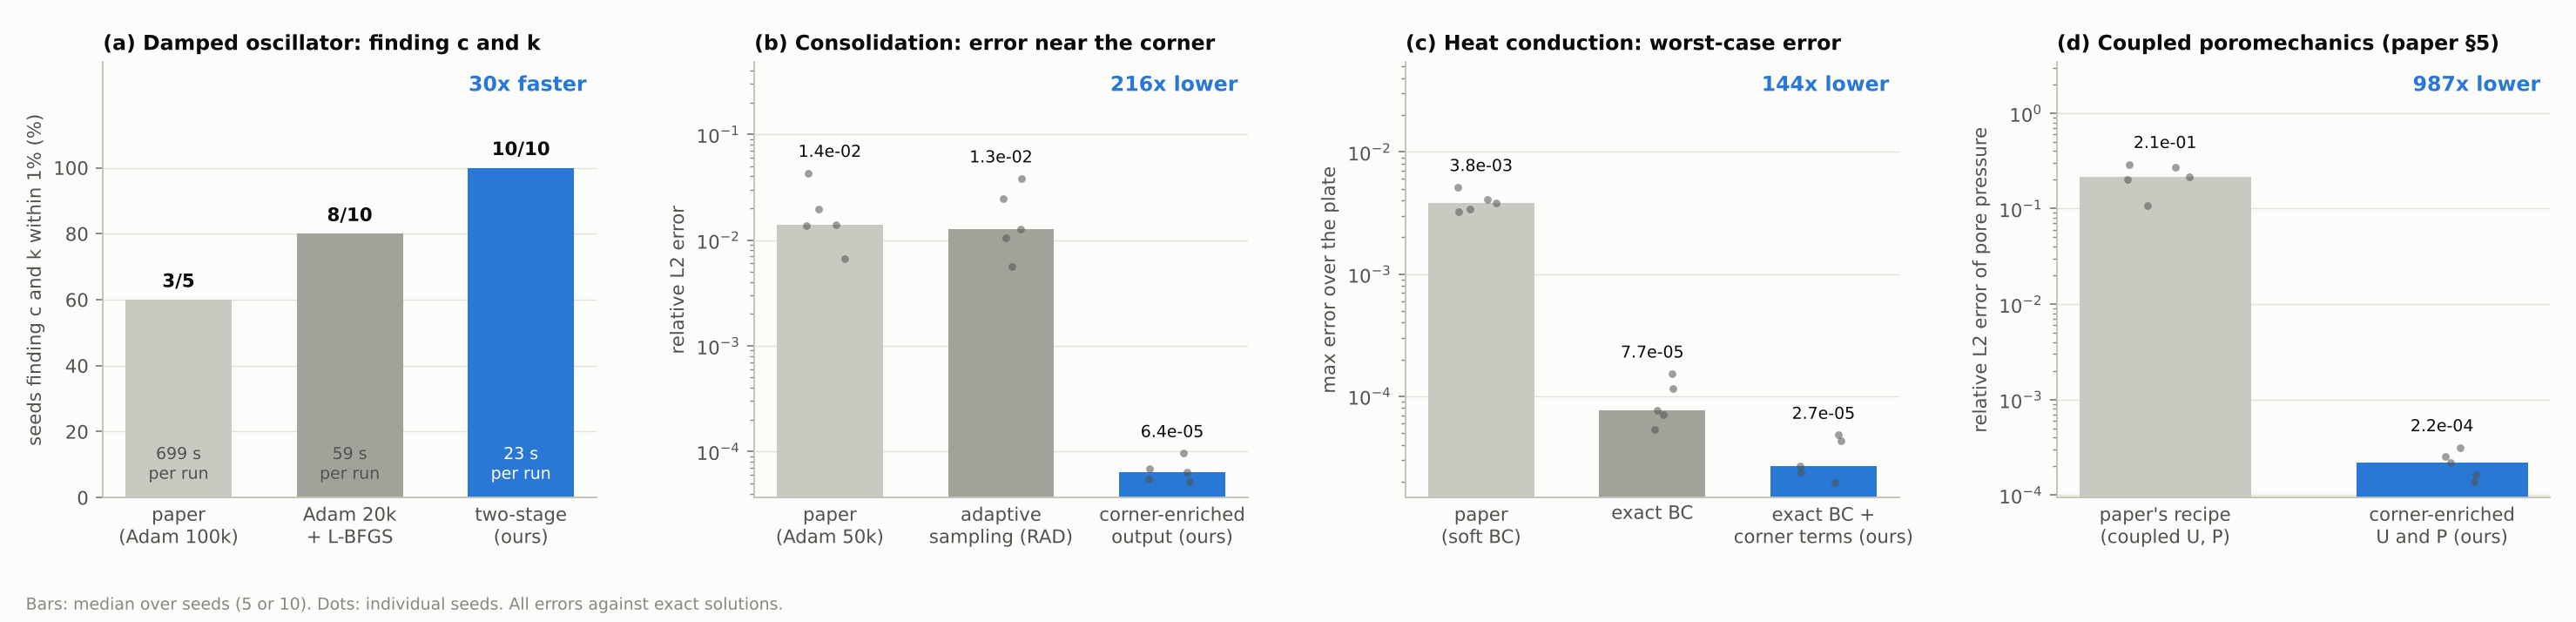
\includegraphics[width=\linewidth]{../../results/figures/summary.png}
\captionof{figure}{Paper's method (grey) vs our fixes (blue). Bars: median over seeds; dots: individual seeds.}
\end{center}
\vspace{-4pt}
\begin{enumerate}[label=\textbf{\arabic*.}]
\item \textbf{One run is not evidence.} The paper's accuracy holds for some seeds and not others.
\item \textbf{Training loss can mislead.} Near corners the loss looked converged while the equation was badly violated;
residuals on fresh points exposed it every time.
\item \textbf{Put known structure in the output, not the loss.} Exact boundary conditions and analytical enrichment
beat adaptive sampling and longer training, and the same idea solved the paper's future-work problem.
\item \textbf{Warm starts make inverse problems reliable}, from 3/5 to 10/10 seeds at 30$\times$ the speed.
\item \textbf{A PINN is not always the right tool.} With a known closed form and two parameters, a classical fit
matches or beats it; PINNs earn their place when data are incomplete and physics must fill the gaps.
\end{enumerate}
\textbf{Limitations.} Enrichment terms need analytical insight into each problem; uncertainty estimates for
discovered parameters are future work. Full details are in the 16-page report and the repository README.

\end{document}
